\documentclass{article}
\usepackage{geometry}
\usepackage{amsmath}
\usepackage{amssymb}
\usepackage{tabularx}
\usepackage[table]{xcolor}
\usepackage{tikz}
\usetikzlibrary{quantikz}
\usepackage{graphicx}      % For including graphics
\usepackage{subcaption}    % For subfigures


% Tables
\usepackage{booktabs}      % For better table rules
% Define custom colors
\definecolor{headerblue}{RGB}{176,196,222}   % Light steel blue for header
\definecolor{rowblue}{RGB}{224,236,240}      % Very light grey-blue for alternating rows


\usepackage{bbm}

\newcommand{\argmin}{\operatorname*{arg\,min}}
\newcommand{\boldtheta}{\boldsymbol{\theta}}
\newcommand{\vone}{\mathbbm{1}}

\usepackage[backend=biber]{biblatex}
\usetikzlibrary{arrows.meta,positioning,decorations.text}

\title{NeQst -- Kongsberg Use Cases}
\author{Franz Georg Fuchs, Håvard Heitlo Holm, Ruben Pariente Bassa, Alexandra Rylund Glesaaen ++}
\date{November 2022 $\rightarrow$}

\tikzset{
  base/.style={
    draw,
    inner sep=3pt,
    minimum width=2cm,
    align=center,
  },
  component/.style={
    base,
    % text height=height("A"),
    % text depth=depth("g")
  },
  no-branch/.style={
    decoration={
      text along path,
      text format delimiters={[}{]},
      text={[\small]No},
      text align={left indent=0.1cm},
      raise=2pt,
    },
    postaction={decorate},
  },
  yes-branch/.style={
    decoration={
      text along path,
      text format delimiters={[}{]},
      text={[\small]Yes},
      text align={left indent=0.1cm},
      raise=2pt,
    },
    postaction={decorate},
  },
  % main/.style={
  %   fill=SCColour1!20,
  %   text=SCColour1!40!black,
  %   draw=SCColour1!40!black,
  %   semithick,
  % },
  % optional/.style={
  %   dashed,
  %   fill=SCColour1Tri2!20,
  %   text=SCColour1Tri2!40!black,
  %   draw=SCColour1Tri2!40!black,
  % },
  % request/.style={
  %   fill=SCColour1Tetra1!20,
  %   text=SCColour1Tetra1!40!black,
  %   draw=SCColour1Tetra1!40!black,
  % },
  edge/.style={
    >={Stealth[round]},
    semithick,
    shorten <=1pt,
    shorten >=1pt,
  },
  pre/.style={
    edge,<-,
  },
  post/.style={
    edge,->,
  }
}

\addbibresource{bibliography.bib}

\begin{document}

\maketitle

\abstract{
Todo...
}


\section{Introduction and problem description}
\label{sec:intro}

Quantum algorithms have shown good potential for solving quadratic unconstrained binary optimization (QUBO) problems. 
In the following, we consider a specific application of a routing problem, where a central part of the solution strategy is to solve exact cover problems. 
This is an NP-hard combinatorial optimization problem that map to a QUBO, and is therefore an excellent candidate for taking advantage of advancing quantum computing.
 
The challenge we base this study on is to find the lowest cost for moving a
large number of containers. The containers will be located at several different
ports, and needs to be moved to new locations. There will be more containers
than one boat can carry. There might be that if you use one large boat the draft
will force it to take a longer route. A fast boat might be slowed down by speed
limits on narrow paths, and the path might be too long for some boats. Some
times boats have to be moved without cargo to get to a port with containers.
The problem is continuous as there will be new payloads coming all the time,
creating new jobs, but the boats, ports and paths will be static. 



%How many boats, ports and jobs there must be to make the problem interesting is for
% SINTEF to find out. If it turn out that there is need for thousands of boats to
% make the problem hard enough, then this case might be discouraged and we look
% for another problem. Many more parameters may be added as soon as we have found
% the complexity level of the problem. 
\input{figs/path-examples.tex}


% \section{Simplified path-based model}
To study the potential for solving such optimzation problems with quantum computing, we construct the simplest problem possible that still has some real-world complexity. To start simple we make the paths fixed and finite, such that all routes are
defined with the correct properties. We ignore weather and other boats at first.
A list containing possible model extensions are given in Appendix \ref{app:extended-model} for future references.

The task is to find the optimal use of a set of boats to carry out a set of orders consisting of moving parcels/containers between predefined ports.
We represent the geographical map as a directed graph where the nodes $P$ are the ports and values at the edges represent distance $d_{A,B}$ from port $A$ to port $B$ for $A, B \in P$. Due to prevailing currents/winds or restrictions on boat traffic in areas with many small islands and straights, the distance between two ports might be difference depending on the direction one is traveling, meaning that $d_{A, B} \neq d_{B, A}$. Even more, there might be more than one route between ports, where different routes are better suited for different boats.
% The orders are specified using the following parameters.

% \noindent
% \textbf{Order: }    

% \begin{tabular}{rl}
%     From & Pick-up location \\
%     To & Destination \\
%     Weight & Container weight, or how much resources the order takes from the boat's capacity\\
% \end{tabular}
% \vspace{1em}

For order $o \in O$, we have the following information:

\begin{tabular}{ll}
    $p^{\text{start}}_o$ & Pick-up location $p^{\text{start}}_o \in P$ for order $o$ \\
    $p^{\text{end}}_o$ & Destination $p^{\text{end}}_o \in P$ for order $o$ \\
    $w_o$ & weight of containers in order $o$ [kg]
\end{tabular}
\vspace{1em}


\noindent Furthermore, each boat $b \in B$ has parameters

\begin{tabular}{ll}
    $v_b$ & Average speed of boat $b$ \\
    $K_b$ & Capacity of the boat   \\
    $\Gamma_b$ & Cost per km for sailing boat $b$ \\
    $\gamma_b$ & Cost per load per km for boat $b$ 
\end{tabular}
\vspace{1em}

\noindent This means that if boat $b$ travels from port $A$ to $B$ while it is loaded with containers from orders $\tilde{O} \subset O$, the cost for this transport stage becomes $\left[ \Gamma_b + \gamma_b\sum_{o \in \tilde{O}} w_o\right] d_{A,B}$.



\subsection{Classical solution using a path-based optimization problem}
In the following, we sketch out the classical solution strategy for this optimization problem. To seek optimal use of the resources (boats), we need to support the possibility that a boat can pick new orders before delivering orders it already carries, as long as it is within the boat's capacity. In other words, it is not enough to assign orders between boats, but also to find the shortest path through the graph to pick up and deliver the orders within the capacity constraints of each boat.

We therefore formulate the optimization problem by encoding the information in routes $r$ with associated cost $c_r$. A route is a chronological set of activities for a single boat. An activity can  be to pick up order, travel between ports, and deliver order. This means that a route can include an arbitrary number of orders (also zero), but always one and only one boat. Note however that we can define multiple routes that carry out the same orders with the same boat, for example by taking different paths between a pick-up location and the destination, or carrying out two orders in opposite order.

By writing up all (reasonable) candidate routes $R$ for a set of orders $O$ and set of boats $B$, we can formulate a binary optimization problem. 
\begin{subequations}
    \begin{align}
      \text{min} &\; \sum_{r \in R} c_r x_r \label{eq:path-1}\\
      \text{s.t.}& \; \sum_{r \in R} \tilde{y}_{or} x_r = 1, \hspace{1em} \forall \; o \in O, \label{eq:path-order} \\
      \text{s.t.}& \; \sum_{r \in R} \tilde{y}_{br} x_r = 1, \hspace{1em} \forall \; b \in B, \label{eq:path-boat} \\
       &x_r \in \{0, 1\}, \label{eq:path-3}
    \end{align}
    \label{eq:path}
\end{subequations}
where
\vspace{1em}

\begin{tabular}[c]{ll}
  $R$: & all candidate routes a boat can take \\
  $O$: & all orders of the problem \\
  $B$: & all boats available \\
  $x_r$: & $1$ if we include route $r$ in the solution, $0$ otherwise \\
  $c_r$: & cost of route $r$ \\
  $\tilde{y}_{or}$: & $1$ order $o$ is included in route $r$, $0$ otherwise \\
  $\tilde{y}_{br}$: & $1$ if boat $b$ carries out route $r$, $0$ otherwise \\
\end{tabular}
\vspace{1em}

Here, the constraint \eqref{eq:path-order} ensures that each order is carried out once and only once, and \eqref{eq:path-boat} that each boat is used for one and only one route. By defining a combined column vector $y_r = [\tilde{y}_{br} \, ; \, \tilde{y}_{or}]^T$ and an index $i \in O \cup B$, we can restate the problem as
\begin{subequations}
    \begin{align}
      \text{min}& \; \sum_{r \in R} c_r x_r \label{eq:compact-path-1}\\
      \text{s.t.}& \; \sum_{r \in R} y_{ir} x_r = 1, \hspace{1em} \forall \; i \in O \cup B, \label{eq:compact-path-2} \\
      &x_r \in \{0, 1\}, \label{eq:compact-path-3}
    \end{align}
    \label{eq:compact-path}
\end{subequations}
In general terms, \eqref{eq:compact-path} is called an exact cover (EC) problem.

The solution to the optimization problem describes then the set of routes that carry out all orders once and only once at the lowest cost. This includes which boats to use for which orders and which path to take, along with the associated cost and duration. 


\subsection{Column generation}

An issue with the path model in \eqref{eq:compact-path-1} is that we need to enumerate
every possible routes $r$, and as there are exponentially many of them, we get
an exponential number of variables as the problem size increases. This is
usually tacked by a method called \emph{column generation}, where we start with
a smaller set of variables than the full set, then dynamically generate new
variables (routes) iteratively. To do this, we follow the approach from Gronkvist~\cite{gronkvist_phdthesis} as shown in Figure~\ref{fig:column-generation}.

To guide this effort, i.e. generate new routes in a systematic way that leads
towards optimality, we set up the pricing problem. If $\pi_i$ is the dual
variable to the constraints \eqref{eq:compact-path-2}, then the pricing problem is simply
%
\begin{equation}
  \bar{c}_r = c_r - \sum_{i \in O \cup S} y_{ir} \pi_i.
  \label{eq:pricing-problem}
\end{equation}
%
A candidate route is one with a negative reduced cost ($\bar{c}_r$). Any such
route can be added as a column, but it is usually better to find the one that is
the most negative, and possibly more than one at a time. One way to find these
routes is to see the pricing-problem as a shortest path problem in a graph of
the order/boat $i$ where the node cost is $\pi_i$. This graph, and the possible
the path through it, will be restricted by the constraints of the full problem  such as for boat capacity (or others from Appendix \ref{app:extended-model}).
A shortest path can for instance be found with a labeled
algorithm to get dependencies not in the graph itself.

\begin{figure}
\begin{center}
  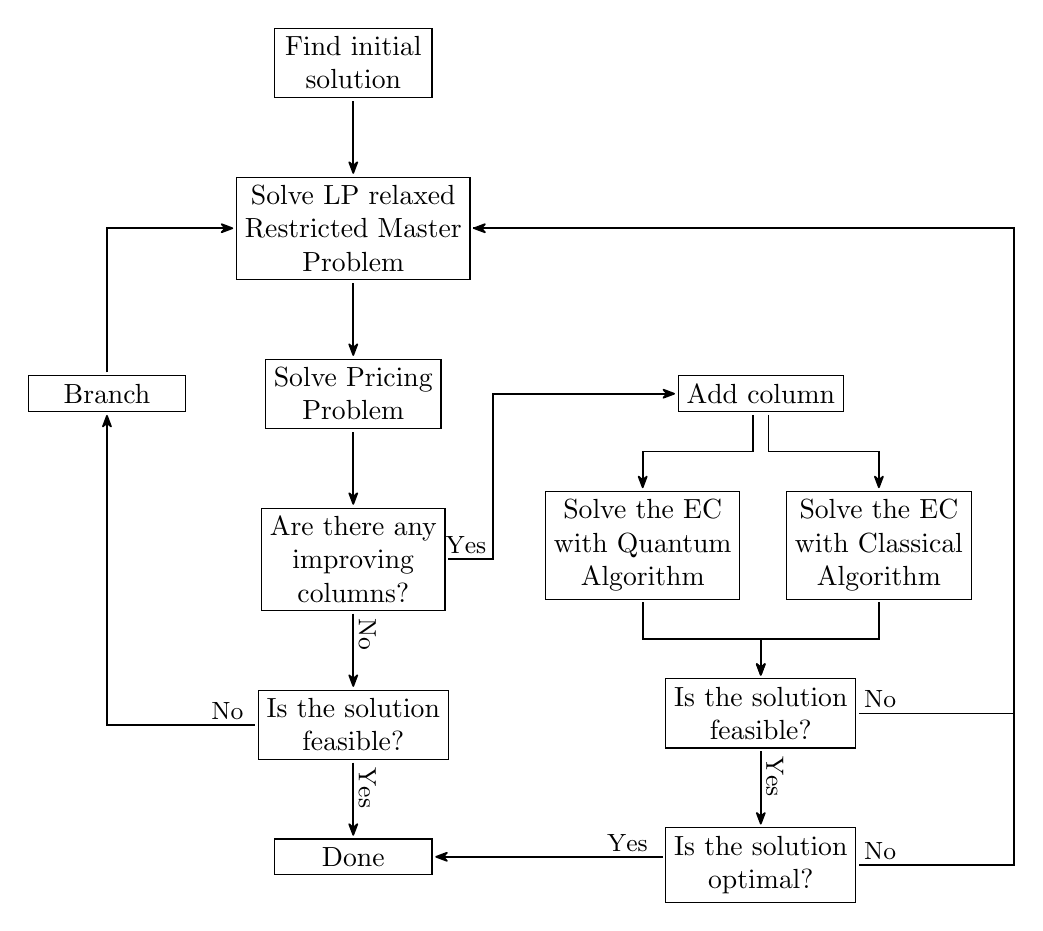
\begin{tikzpicture}
    \node [component] (init) {Find initial\\solution};
    \node [component, below=1cm of init] (relax)
      {Solve LP relaxed\\Restricted Master\\ Problem}
      edge [pre] (init);
    \node [component, below=1cm of relax] (pricing-problem)
      {Solve Pricing\\Problem}
      edge [pre] (relax);
    \node [component, below=1cm of pricing-problem] (new-colums)
      {Are there any\\improving\\columns?}
      edge [pre] (pricing-problem);
    \node [component, below=1cm of new-colums] (pp-feasible)
      {Is the solution\\feasible?};
\node [component, below=1cm of pp-feasible] (done)
      {Done};

    \node [component, left=1cm of pricing-problem] (branch)
      {Branch};

    % Right branch
    \node[component, right=3cm of pricing-problem] (add-col) {Add column};
    \node [component, below=1cm of add-col, xshift=-1.5cm] (rmp-quantum)
      {Solve the EC\\with Quantum\\Algorithm};
    \node [component, below=1cm of add-col, xshift=1.5cm] (rmp-classical)
      {Solve the EC\\with Classical\\Algorithm};
    \node [component, below=1cm of rmp-quantum, xshift=1.5cm] (rmp-feasible)
      {Is the solution\\feasible?};
    \node [component, below=1cm of rmp-feasible] (rmp-optimal)
      {Is the solution\\optimal?};

    % Left branch edges
    \draw[
      edge, ->,
      decoration={
        text along path,
        text format delimiters={[}{]},
        text={[\small]Yes},
        text align={left},
        raise=2pt,
      },
      postaction={decorate},
    ] (new-colums.east) -- +(0.6,0) |- (add-col.west);

    \draw[edge, ->, no-branch] (new-colums.south) -- (pp-feasible.north);
    \draw[edge, ->, yes-branch] (pp-feasible.south) -- (done.north);

    \draw[
      edge, <-,
      decoration={
        text along path,
        text format delimiters={[}{]},
        text={[\small]No},
        text align={left indent={0.9\dimexpr\pgfdecoratedpathlength\relax}},
        raise=2pt,
      },
      postaction={decorate},
    ] (branch.south) |- (pp-feasible.west);
    \draw[edge, ->] (branch.north) |- (relax.west);

  % Right branch edges
    \draw[edge, ->] ([xshift=-0.1cm] add-col.south) -- +(0, -0.5cm) -| (rmp-quantum.north);
    \draw[edge, ->] ([xshift=0.1cm] add-col.south) -- +(0, -0.5cm) -| (rmp-classical.north);
    
    \draw[edge, ->] (rmp-quantum.south) -- +(0, -0.5cm) -| (rmp-feasible.north);
    \draw[edge, ->] (rmp-classical.south) -- +(0, -0.5cm) -| (rmp-feasible.north);

    \draw[edge, ->, yes-branch] (rmp-feasible.south) -- (rmp-optimal.north);
    \draw[
      edge, <-,
      decoration={
        text along path,
        text format delimiters={[}{]},
        text={[\small]Yes},
        text align={left indent={0.75\dimexpr\pgfdecoratedpathlength\relax}},
        raise=2pt,
      },
      postaction={decorate},
    ] (done.east) -- (rmp-optimal.west  |- done.east);

    \draw[edge, no-branch] (rmp-feasible.east) -- +(2cm, 0) |- (relax.east);
    \draw[edge, ->, no-branch] (rmp-optimal.east) -- +(2cm, 0) |- (relax.east);
    
  \end{tikzpicture}
\end{center}
\caption{Workflow for solving the path-based optimization problem using column generation.}
\label{fig:column-generation}
\end{figure}

In this workflow, and for large problem instances in particular, we assume that column generation is an easy task, whereas solving the EC problem is hard. We therefore focus our attention to how we can use quantum computing to solve the EC problem with routes (columns) generated from the shipping problem.

\section{Quantum algorithm to solve the exact cover problem}
Here, we will outline the basic steps for solving the exact cover problem using the quantum approximate optimization algorithm (QAOA)~\cite{hadfield2019_qaoa2qaoa},  which is a generalization to the quantum approximate optimization algorithm~\cite{farhi2014QAOA}. We will also discuss how we can take advantage of properties of the specific exact cover problems that occurs from the path-based optimization problem.

\subsection{Quantum approximate optimization algorithm}

Our strategy is to re-formulate the EC problem from \eqref{eq:compact-path} to a quadratic unconstrained binary optimization (QUBO) problem, defined as 
\begin{subequations}
    \begin{align}
      \text{min}& \; x^T Q x + w^T x \label{eq:qubo-min}\\
      \text{with} \; x \in \{0, 1\}^n, & \quad Q \in \mathbb{R}^{n\times n}, \quad w \in \mathbb{R}^n. \label{eq:qubo-const}
    \end{align}
    \label{eq:qubo}
\end{subequations}
It is well-known that QUBO cost functions $C(x)$ on the form of \eqref{eq:qubo-min} can be mapped to a Hamiltonian operator $H_c$, so that the minimum value of $C(x)$ corresponds to the minimum energy of $H_c$.
By writing the cost function as
\begin{equation}
    C(x) = \sum_{i,j=1}^n x_i Q_{i,j} x_j + \sum_{i=1}^n w_i x_i,
    \label{eq:qubo-cost-fun}
\end{equation}
there is a corresponding Hamiltonian operator
\begin{equation}
    H_c = \sum_{i,j=1}^n \frac{1}{4}Q_{i,j}Z_i Z_j - \sum_{i=1}^n \frac{1}{2}\left( w_i + \sum_{j=1}^n Q_{i,j} \right)Z_i + \left( \sum_{i,j=1}^n \frac{1}{4}Q_{i,j} + \sum_{i=1}^n \frac{1}{2}w_i\right),
    \label{eq:hamiltonian}
\end{equation}
where $Z$ is Pauli basis function.

\begin{figure}
    \centering
    \begin{quantikz}[row sep={0.7cm,between origins}]
    \lstick{$q_1$} & \gate[5]{U_0} & \gate[5]{U_c(\gamma_1)} & \gate[5]{U_M(\beta_1)} & \qw & &  &\gate[5]{U_c(\gamma_P)} & \gate[5]{U_M(\beta_P)} & \meter{} \\
    \lstick{$q_2$} & &  & & \qw  & & & &  & \meter{} \\
    \lstick{$q_3$} & &  &  &  \qw  &\ldots\ & & &  & \meter{} \\
    \lstick{$\vdots$} & &  & & \qw  & & & &  & \meter{} \\
    \lstick{$q_n$} & &  & & \qw  & & & &  & \meter{} \\
    \end{quantikz}
    \caption{Quantum circuit structure with initial unitary $U_0$, alternating cost and mixer unitaries $U_c(\gamma_j)$ and $U_M(\beta_j)$ for $j = 1,\dots,P$, followed by measurements.}
    \label{fig:qaoa-circuit}
\end{figure}

To find the minimum energy of the Hamiltonian $H_c$ we will use the QAOA, which is a generalization to the quantum approximate optimization algorithm \cite{hadfield2019_qaoa2qaoa}. 
This method consists of constructing a parameterized quantum circuit as depicted in Figure~\ref{fig:qaoa-circuit}. The circuit consists of an initialization operator, followed by $P$ layers of alternating cost operators and mixer operators.
The cost unitary operator is given by 
\begin{equation}
    U_c(\gamma_j) = e^{-i \gamma_j H_c}, \qquad j=1,..., P,
    \label{eq:cost_operator}
\end{equation}
and encodes the objective function from the optimization problem into the quantum state, so that its energy reflects the associated cost value.
The mixer operator applies parameterized rotations to the quantum state, thereby exploring the solution space and avoiding that the algorithm gets stuck at local minima. It is given by
\begin{equation}
    U_M(\beta_j) = e^{-i \beta_j H_M}, \qquad j=1,..., P,
    \label{eq:mixer_operator}
\end{equation}
where $H_M$ is a mixer Hamiltonian.

Denoting the QAOA parameters by $\boldtheta_P = \{\gamma_j, \beta_j\}_{j=1}^{P}$, we can express the circuit as
\begin{equation}
    |\psi(\boldtheta_P)\rangle =
U_M(\beta_P)\, U_C(\gamma_P)\, \cdots \, U_M(\beta_1)\, U_C(\gamma_1)\, U_0\, |\psi_0\rangle.
    \label{eq:qaoa-circ}
\end{equation}
The goal then is to find the parameters $\boldtheta_P$ that minimizes the energy in the Hamiltonian, and thereby minimizes the cost function. The hypothesis is that this is easier and/or faster than solving the given optimization problem directly using classical algorithms.

Although evaluating the QAOA circuit in \eqref{eq:qaoa-circ} requires a (simulated) quantum computer, the optimization algorithm for finding optimal circuit parameters is classical. Here, it is possible to use a wide variety of classical optimization algorithms, with the objective to minimize a statistical cost function $f(\boldtheta_P)$. By evaluating and measuring $|\psi(\boldtheta_P)\rangle$ $M$ times in the computational basis to obtain candidate solutions $\{x_i\}_{i=1}^M$, we can define this cost function to be the mean of the associated QUBO costs from \eqref{eq:qubo},
\begin{equation}
    f(\boldtheta_P) = \frac{1}{M}\sum_{i=1}^{M} C(x_i).
    \label{eq:circuit_mean}
\end{equation}

An alternative statistical evaluation metric of the QAOA circuit, is to use the conditional value at risk (CVaR), which has been demonstrated to increase the performance of such variational quantum algorithms~\cite{Barkoutsos2020improving}. By specifying a CVaR confidence level $\alpha \in (0, 1]$ we only consider the $\alpha$-fraction of the best candidate solutions. This means that if the set of candidate solutions $\{x_i\}_{i=1}^M$ is sorted so that $C(x_i) \leq C(x_j)$ for all $i < j$, the CVaR is given as
\begin{equation}
    f_{\alpha}(\boldtheta_P) = \frac{1}{\lceil \alpha M \rceil}\sum_{i=1}^{\lceil \alpha M \rceil} C(x_i).
    \label{eq:circuit_cvar}
\end{equation}
Note that \eqref{eq:circuit_cvar} becomes equal to \eqref{eq:circuit_mean}  when $\alpha = 1$.

In practice, it is hard to find optimal parameters for the QAOA circuit by directly exploring the parameter space of a full $P$-layered circuit. Instead, it is common to start finding the two optimal parameters for a one layered circuit, then iteratively expand the parameter search and circuit by adding a new layer using the previous optimal parameters to construct well-informed initial guesses. 


\subsection{Reformulating the exact cover as a QUBO}

To solve our path-based shipping problem using QAOA we first need to reformulate the EC problem in \eqref{eq:compact-path} to a QUBO on the form of \eqref{eq:qubo}. We start by writing \eqref{eq:compact-path} on vectorized form.

First, for a given EC problem, we denote the number of orders, boats, and possible routes as $N_o$, $N_b$, and $N_r$, respectively. Then, we introduce the coverage matrix $Y$ consisting of $N_r$ columns and $N_b + N_o$ rows.
This means that each column represents a route, while the $N_b$ top rows represent which boat to use and the bottom $N_o$ rows represent the which orders the route will cover.
Furthermore, we will have a weight vector $c \in \mathbb{R}^{N_r}$ representing the cost associated to route each route, and the binary state variable $x \in \{0, 1\}^{N_r}$ indicating which routes we be included in the solution.
We can then rewrite \eqref{eq:compact-path} as
\begin{subequations}
    \begin{align}
      \text{min}& \; c^T x \label{eq:vectorized-ec-1}\\
      \text{s.t.}& \; Y x = \mathbbm{1}. \label{eq:vectorized_ec-2}
    \end{align}
    \label{eq:vectorized_ec}
\end{subequations}
In other terms, we want to find $x^{\star}$ that is the solution to
\begin{equation}
     x^\star = \argmin_{||Y x - \mathbbm{1}||_2 = 0} \left\{ c^T x \right\}.
     \label{eq:standard-ec}
\end{equation}

Although \eqref{eq:standard-ec} is a binary optimization problem, it is not unconstrained. 
To get rid of the constrain, we introduce a suitable penalization factor $\lambda$, chosen such that the solution of \eqref{eq:standard-ec} is also the solution of
\begin{equation}
    x^\star = \argmin \left\{ c^T x + \lambda ||Y x - \mathbbm{1}||_2^2 \right\}.
    \label{eq:ec-vec}
\end{equation}
By expanding the penalization term, we get
\begin{equation}
    x^\star = \argmin \left\{ c^T x + \lambda \left((Yx)^T (Yx) - 2\lambda \vone^T(Yx) + \vone^T \vone \right) \right\}.
    \label{eq:ec-qubo-full}
\end{equation}
By sorting the terms, we see that we can write \eqref{eq:ec-qubo-full} as the QUBO
\begin{equation}
    x^\star = \argmin \left\{ x^T Q x + w^T x + b \right\},
    \label{eq:ec-qubo}
\end{equation}
with
\begin{subequations}
    \begin{align}
      Q =& \lambda Y^T Y, \label{eq:ec-qubo-coeffs-1}\\
      w =& c^T  - 2 \lambda \vone^T Y, \label{eq:ec-qubo-coeffs-2}\\
      b =& \vone^T \vone = N_o + N_b. \label{eq:ec-qubo-coeffs-3}
    \end{align}
    \label{eq:ec-qubo-coeffs}
\end{subequations}
which is equivalent to \eqref{eq:qubo} since the constant $b$ does not alter the solution to the minimization problem.


\subsection{Solving the exact cover problems using QAOA}
\label{sec:ec-pruning}

We will now look into how to modify the exact cover problems to make it easier to solve by analysing the forms they take when arising from the path-based column generation. 
Although \eqref{eq:ec-qubo} and \eqref{eq:ec-qubo-coeffs} are important as they show us how to map the problem to the Hamiltonian operator from \eqref{eq:hamiltonian}, we will continue discussing the exact cover problems in terms of \eqref{eq:ec-vec}.


\subsubsection{General bound for penalization factor}
\label{sec:ec-orig}
\begin{description}
    \item[Goal:] Ensure that all infeasible solutions are worse than all feasible solutions.
\end{description}
The first task for solving \eqref{eq:ec-vec} is to specify the value for the penalization factor $\lambda$. In general, we gave to find a trade-off that balances feasibility and optimality~\cite{Wang2020-XYmixers}. On one hand, we have to construct $\lambda$ so that any infeasible solution are always worse than the best feasible solutions. On the other, we want to avoid setting $\lambda$ larger than necessary, as this often leads to a staircase-formed cost landscape, which is harder for optimization algorithms. 

For an infeasible solution of the exact cover problem \eqref{eq:ec-vec}, the term $||Y x - \mathbbm{1}||_2^2$ has a lower bound at 1. In the worse case, consider a problem where only a few of the elements of $c$ are non-zero and they are all part of the only solution to the problem, while all other elements are zero. In this case, an infeasible solution where all associated costs are zero, requires that
\begin{equation}
    \lambda > \sum_{i=1}^{N_r} \max(0, c_i).
    \label{eq:lambda-general}
\end{equation}


\subsubsection{Subset with all feasible solutions}
\label{sec:ec-subset}
\begin{description}
    \item[Goal:] Avoid searching for solutions where there for sure are none. 
\end{description}
Until now, we have been searching for a solution to the exact cover problem in the space
\begin{equation}
    S = \left\{ x \in \{0,1\}^{N_r} \right\},
    \label{eq:total-solution-space}
\end{equation}
where there are a total of $|S| = 2^{N_r}$ candidate solutions.
Now, we take advantage of a specific property for our problem. Since each route (column in $Y$) describes which orders are handled a given boat, all valid columns of $Y$ will have a single one-valued element among its $N_b$ first rows. This means, that all feasible solutions to the exact cover problem must be represented by $N_b$ routes. Therefore, we can safely search for solutions within the subspace 
\begin{equation}
    S_f = \left\{x \in \{0,1\}^{N_r} : |x| = N_b\right\},
    \label{eq:feasible_space}
\end{equation}
and replace \eqref{eq:ec-vec} by
\begin{equation}
    x^\star = \operatorname*{arg\,min}_{ |x| = N_b} \left\{ c^T x + \lambda ||Y x - \mathbbm{1}||_2^2 \right\}.
    \label{eq:ec-subspace}
\end{equation}
This constrain is referred to as a "$k$-hot", or a states with a Hamming weight of $N_b$.  
By introducing this constraint, we effectively reduces the size of our search space from $2^{N_r}$ to only $|S_f| = \binom{N_r}{N_b}$.

To take advantage of the known Hamming weight of the solution, we need to modify the QAOA algorithm in two ways.
First, we construct $U_0$ in \eqref{eq:hamiltonian} so that it initialize QAOA using a Dicke state, which prepares a quantum state with a given number of non-zero values. 
Second, we use a suitable subspace-preserving mixer (see, e.g.,~\cite{Fuchs2022_cp-mixers, Fuchs2024lxmixersqaoa}) that ensures that the QAOA circuit only explores solutions with the given Hamming weight. To this end, we can either use a $XY$-mixer~\cite{hadfield2017_qaoaHardSoft, Wang2020-XYmixers} or a Grover mixer~\cite{Bartschi2020_groverMixer}.


\subsubsection{Better bound for penalization factor}
\label{sec:ec-penalty}
\begin{description}
    \item[Goal:] Ensure all infeasible solutions with Hamming weight $H_b$ are worse than all feasible solutions.
\end{description}

Using the constraint in \eqref{eq:ec-subspace}, we can now tighten the bound on the penalization factor by realizing that we only have to account for the gap between the worst and best possible costs for states with Hamming weight $N_b$. This means we now can choose $\lambda$ by requiring
\begin{equation}
    \lambda >  \max_{|x| = N_b}\left\{ c^T x \right\}  - \min_{|x| = N_b}\left\{ c^T x \right\}.
    \label{eq:lambda-specific}
\end{equation}


\subsubsection{Scaling}
\label{sec:ec-scaled}
\begin{description}
    \item[Goal:]  Ensure that all possible solutions (both feasible and infeasible) are between 0 and $2\pi$, and that we facilitate for the potential of using the entire interval.
\end{description}
We start with the second part of this goal that ensures that the smallest possible feasible solution gives a cost close to zero. 
Due to the constraint $|x| = N_b$, we observe that $\mathbbm{1}^T x = N_b$ for any feasible $x$. We can therefore alter our original cost function by adding any constant $a$ so that
\begin{equation}
    \argmin_{|x| = N_b}\left\{ c^T x \right\} = \argmin_{|x| = N_b}\left\{ c^T x - a\right\} = \argmin_{|x| = N_b}\left\{ \left(c - \frac{a}{N_b}\mathbbm{1}\right)^T x \right\}.
    \label{eq:cost-scaling-1}
\end{equation}
By letting $a$ be the lower bound of the cost function, which is the sum of the $N_b$ smallest weights $a = \min_{|x| = N_b}\left\{ c^T x \right\}$, and by introducing $\omega = c - a/N_b$, we ensure that the lower bound of the cost function $f_{\omega}(x) = \omega^T x$ is zero for all $|x| = N_b$.
The solution to our problem is still the same, meaning that we now have
\begin{equation}
    x^\star = \argmin_{ |x| = N_b} \left\{ \omega^T x + \lambda ||Y x - \mathbbm{1}||_2^2 \right\},
    \label{eq:cost-scaling-2}
\end{equation}
where the penalization factor is simplified to
\begin{equation}
    \lambda > \max_{|x| = N_b}\left\{ \omega^T x \right\}.
    \label{eq:scaling-penalty-1}
\end{equation}

To restrict the upper bound on the penalized optimization problem in \eqref{eq:cost-scaling-2}, we seek a scaling parameter $b$ which we can tune to ensure an upper bound of the cost function in
\begin{equation}
    x^{\star} = \argmin_{ |x| = N_b} \left\{ b \left( \omega^T x  + \lambda ||Y x - 1||^2_2 \right)\right\}.
    \label{eq:cost-scaling-3}
\end{equation}
The upper bound for the first term is already known as $\omega^T x \leq \max_{|x| = N_b}\left\{ \omega^T x \right\}$.

For the upper bound for the penalty term, we first note that $Y x$ has $N_o + N_b$ elements, for which each element can have a integer value between 0 and $N_b$. Since we assume that $N_b$ will be at least 2 (otherwise, the problem is trivial), each element of $Y x - 1$ will be at worst $N_b - 1$.
This means that $||Y x - 1||^2_2 \leq (N_o + N_b)(N_b - 1)^2$.

For the penalized problem, which we want to be smaller than $2 \pi$, we then get

\begin{equation}
    \begin{split}
     2\pi \leq&\, b\left(\omega^T x + \lambda ||Y x - 1||^2_2 \right) \\
        \leq&\, b\left(\max_{|x| = N_b}\left\{ \omega^T x \right\} + \lambda (N_o + N_b)(N_b - 1)^2 \right)\\
        \approx&\, b\left(\max_{|x| = N_b}\left\{ \omega^T x \right\} \left[ 1 + (N_o + N_b)(N_b - 1)^2 \right]\right).
    \end{split}
\end{equation}
At the final step, we have assumed that the penalty term from \eqref{eq:scaling-penalty-1} is set as low as possible.

In summary, we get the following scaled problem:
\begin{equation}
    x^{\star} = \argmin_{ |x| = N_b} \left\{ b \left( \omega^T x  + \lambda ||Y x - 1||_2 \right)\right\},
    \label{eq:scaled-ec}
\end{equation}
with scaled weight vector
\begin{equation}
    \omega = c - \frac{1}{N_b} \min_{|x| = N_b}\left\{ c^T x \right\}, 
    \label{eq:scaled-cost-vector}
\end{equation}
penalty term
\begin{equation}
    \lambda > \max_{|x| = N_b}\left\{ \omega^T x \right\},
    \label{eq:scaled-penalty}
\end{equation}
and global scaling
\begin{equation}
    b = 2 \pi \left(\max_{|x| = N_b}\left\{ \omega^T x \right\} \left[ 1 + (N_o + N_b)(N_b - 1)^2 \right]\right)^{-1}.
    \label{eq:scaled-scale}
\end{equation}


\section{Experimental results}
Here, we define the problem instances, and discuss experimental results using simulated quantum circuits. We do this by constructing different cases of the path-based problems by defining number of boats, ports, and orders, and then use column generation to generate exact cover problems that we solve classically. This gives us a set of test problems for our quantum problem for each of the path-based problems.

\subsection{Case A: 2 boats, 3 ports, 3 orders}
We start by looking at a very small problem consisting of 2 boats, 3 ports, and 3 orders. Through column generation we obtain eight exact cover problems as listed in Table~\ref{tab:caseA}. Note that the number of qubits required for each problem is equal to $N_r$. Note also how much we restrict the solution search space when going from $S$ to $S_f$ when considering only solutions with a given Hamming weight.


\begin{table}
\centering
\rowcolors{2}{rowblue}{white} % Alternating row colors starting from row 2
\begin{tabular}{r c r r c}
\rowcolor{headerblue!80} % Header row color
{\textbf{Case Name}} & 
{\textbf{$N_r$}} & {\textbf{$|S|$}} & 
{\textbf{$|S_f|$}} & {\textbf{\# feasible solutions}}  \\
\midrule
EC-A1 & 7 & 128 & 21 & 2 \\
EC-A2 & 4 & 16 & 6 & 2 \\
EC-A3 & 6 & 64 & 15 & 2 \\
EC-A4 & 8 & 256 & 28 & 2 \\
EC-A5 & 10 & 1\,024 & 45 & 2 \\
EC-A6 & 12 & 4\,096 & 66 & 4 \\
EC-A7 & 14 & 16\,384 & 91 & 6 \\
EC-A8 & 14 & 16\,384 & 91 & 6 \\
\end{tabular}
\caption{The exact cover problems occurring from column generation for Case A.}
\label{tab:caseA}
\end{table}

For this very small case, our goal is to investigate how to configure QAOA to solve the exact cover problems that occurs in the path-based problem. There are especially three factors that has to be tuned, and to investigate each of them, the best configuration from the other two factors are needed.
These factors and their best configurations are:
\begin{enumerate}
    \item Problem formulation as discussed in Section~\ref{sec:ec-pruning}, where the final scaled formulation from Section~\ref{sec:ec-scaled} proves to give best results.
    \item Which mixer to use, where the Grover mixer gives much better results than the $XY$-mixer.
    \item Value for CVaR when assessing the cost function from \eqref{eq:circuit_cvar} used to optimize the QAOA parameters. Unless otherwise stated, we will use a CVaR parameter $\alpha = 0.7$.
\end{enumerate}
In the following, we will assess each of these factors in turn.

\subsubsection{Problem formulation}
% Generated from NeQst-WP1/kongsberg/kongsberg/notebooks/PostProcessAllProbs.ipynb
% for input folder:
% result_folder = os.path.join("results", "251008-123112-result_2B_3O_3P")

Figure~\ref{fig:ECA6} shows the results of running QAOA for different configurations of the exact cover problem, using the EC-A6 problem instance as an example. The different configurations are defined as follows:
\begin{description}
    \item[original] The original formulation of the penalized exact cover problem where the solutions from the complete solution space $S$ is considered (see Section~\ref{sec:ec-orig}).
    \item[subset] When enforcing the restriction $|x| = N_b$ to search for solutions only in the subset $S_f$ (see Section~\ref{sec:ec-subset}).
    \item[penalty] Tightening the bound for the penalization factor according to \eqref{eq:lambda-specific} (see Section~\ref{sec:ec-penalty}).
    \item[scaled] After also scaling the range of the penalized cost function to the interval $[0, 2\pi]$ according to equations \eqref{eq:scaled-ec} to \eqref{eq:scaled-scale} (see Section~\ref{sec:ec-scaled}).
\end{description}
The hit ratio is defined as the fraction of shots (individual evaluations of the quantum circuit) that finds the optimal solution of the exact cover problem using the best obtained parameters after each depth iteration in QAOA. The dotted lines show expected hit ratios if we were to sample random solutions from the complete solution space $S$ (blue) and the $k$-hot subset space $S_f$ (orange).
Results from both Figures~\ref{fig:ECA6-orig} and \ref{fig:ECA6-subset} shows poor results, where the hit ratios after optimizing the QAOA parameters are similar to randomly sampling from all considered solutions. After applying scaling, however, Figure~\ref{fig:ECA6-all} we get significantly better results, as approximately every third shot points to the optimal solution. This indicates how crucial it is to scale the range of the cost function for obtaining any results from QAOA.

\begin{figure}
\centering
\begin{subfigure}[b]{0.32\textwidth}
    \includegraphics[width=\textwidth]{figs/eca6-orig.pdf}
    \caption{}
    \label{fig:ECA6-orig}
\end{subfigure}
\hfill
\begin{subfigure}[b]{0.32\textwidth}
    \includegraphics[width=\textwidth]{figs/eca6-subset.pdf}
    \caption{}
    \label{fig:ECA6-subset}
\end{subfigure}
\hfill
\begin{subfigure}[b]{0.32\textwidth}
    \includegraphics[width=\textwidth]{figs/eca6-all.pdf}
    \caption{}
    \label{fig:ECA6-all}
\end{subfigure}
\caption{Hit ratio for optimal solution using optimal parameters found by QAOA using different formulations of the exact cover problem for EC-A6 from Case A.  Here, (a) show the original formulation only, (b) adds results after restricting the search space and improving the penalization, and (c) adds results after scaling the cost function. }
\label{fig:ECA6}
\end{figure}

\subsubsection{Parameter value for CVaR}
% see NeQst-WP1/kongsberg/kongsberg/notebooks/ExactCover_CVaR.ipynb

Here we consider which value of CVaR that seems most promising when using the Grover mixer and the scaled problem formulation.
Figure~\ref{fig:ECA6-cvar} shows the results for the EC-A6 problem instance for a range of CVaR $\alpha$ values, where Figures~\ref{fig:ECA6-cvar-optimal} and \ref{fig:ECA6-cvar-feasible} shows the hit ratio for optimal and feasible solutions, respectively.

The results show that using $\alpha \in (0.5, 0.9)$ seems to be a good choice for finding optimal solutions as all these values find optimal solutions on approximately every third shot. When considering finding feasible solutions, we see a larger spread in the hit ratios, where the interval $\alpha \in (0.7, 0.9)$ seems to be a better choice.
For low values of $\alpha$, we see that the parameter optimizer is unable to obtain better hit ratios larger than $\alpha$ for optimal solutions. This is due to the CVaR cost function reaching its global optimum at this point, meaning that the optimizer has no more information on how to find even better QAOA parameters.
From these results alone, it is hard to point out a single $\alpha$ value that is much better than anything else, but stick to a $\alpha = 0.7$ for our other experiments.

\begin{figure}
\centering
\begin{subfigure}[b]{0.48\textwidth}
    \includegraphics[width=\textwidth]{figs/eca6-cvar-optimal.pdf}
    \caption{}
    \label{fig:ECA6-cvar-optimal}
\end{subfigure}
\hfill
\begin{subfigure}[b]{0.48\textwidth}
    \includegraphics[width=\textwidth]{figs/eca6-cvar-feasible.pdf}
    \caption{}
    \label{fig:ECA6-cvar-feasible}
\end{subfigure}
\caption{Hit ratio for optimal (a) and feasible (b) solutions for exact cover problem instance EC-A6 using different values for CVaR.}
\label{fig:ECA6-cvar}
\end{figure}

\subsubsection{Subset-preserving mixers}
% see NeQst-WP1/kongsberg/kongsberg/notebooks/ExactCover_mixers_cvar07.ipynb
Here, we compare the performance of three types of subspace-preserving mixers for QAOA; the $XY$-mixer with ring topology, the $XY$-mixer with chain topology, and the Grover mixer.
Figure~\ref{fig:ECA6-mixers} shows the results for the EC-A6 problem instance, where Figures~\ref{fig:ECA6-mixers-optimal} and \ref{fig:ECA6-mixers-feasible} shows the hit ratio for optimal and feasible solutions, respectively.

These results clearly shows that the Grover mixer outperforms the $XY$-mixer for both the ring and chain topology. This is the case when considering hit ratio for both the optimal solution and feasible solutions in general.

\begin{figure}
\centering
\begin{subfigure}[b]{0.48\textwidth}
    \includegraphics[width=\textwidth]{figs/eca6-mixers-optimal.pdf}
    \caption{}
    \label{fig:ECA6-mixers-optimal}
\end{subfigure}
\hfill
\begin{subfigure}[b]{0.48\textwidth}
    \includegraphics[width=\textwidth]{figs/eca6-mixers-feasible.pdf}
    \caption{}
    \label{fig:ECA6-mixers-feasible}
\end{subfigure}
\caption{Hit ratio for optimal (a) and feasible (b) solutions for exact cover problem instance EC-A6 using three different subspace-preserving mixers.}
\label{fig:ECA6-mixers}
\end{figure}

\subsubsection{All problem instances}
Finally, using the scaled problem formulation, the Grover mixer, and a CVaR value $\alpha = 0.7$, we evaluate the performance of all the problem instances related to Case A.
Figures~\ref{fig:caseA-optimal} and \ref{fig:caseA-feasible} show the hit ratio for each of the problems for optimal solution and all feasible solutions, respectively.

These results show that after optimizing the QAOA parameters we consistently find optimal solutions for problem instances EC-A1 -- EC-A5 at almost every second shot. For problem instance EC-A7 and EC-A8, which are of the same size, we find optimal solutions on every fifth shot. For all problems, almost all shots are on feasible solutions.
Although these results are quite good, it is obvious from Table~\ref{tab:caseA} that all problem instances here are quite small.


\begin{figure}
\centering
\begin{subfigure}[b]{0.48\textwidth}
    \includegraphics[width=\textwidth]{figs/EC-A-hitratio-optimal-all.pdf}
    \caption{}
    \label{fig:caseA-optimal}
\end{subfigure}
\hfill
\begin{subfigure}[b]{0.48\textwidth}
    \includegraphics[width=\textwidth]{figs/EC-A-hitratio-feasible-all.pdf}
    \caption{}
    \label{fig:caseA-feasible}
\end{subfigure}
\caption{Hit ratio for optimal (a) and feasible (b) solutions for all exact cover problems constructed through Case A.}
\label{fig:caseA-hit-ratios}
\end{figure}

\subsection{Case B: 3 boats, 5 ports, 5 orders}
We now consider a slightly larger problem consisting of 3 boats, 5 ports, and 5 boats. Table~\ref{tab:caseB} shows the number of routes/qubits, and the total and restricted solution spaces for each of them. 
Although the total solution spaces are much larger for this case, we still have relatively small relevant subspaces $S_f$ based on the known Hamming weight of the feasible solutions for these problem instances. 

\begin{table}
\centering
\rowcolors{2}{rowblue}{white} % Alternating row colors starting from row 2
\begin{tabular}{r c r r c}
\rowcolor{headerblue!80} % Header row color
{\textbf{Case Name}} & 
{\textbf{$N_r$}} & {\textbf{$|S|$}} & 
{\textbf{$|S_f|$}} & {\textbf{\# feasible solutions}}  \\
\midrule
EC-B1 & 11 & 2\,048 & 165 & 3 \\
EC-B2 & 6 & 64 & 20 & 3 \\
EC-B3 & 9 & 512 & 84 & 3 \\
EC-B4 & 12 & 4\,096 & 220 & 3 \\
EC-B5 & 15 & 32\,768 & 455 & 3 \\
EC-B6 & 18 & 262\,144 & 816 & 3 \\
EC-B7 & 21 & 2\,097\,152 & 1330 & 3 \\
EC-B8 & 24 & 16\,777\,216 & 2024 & 9 \\
EC-B9 & 26 & 67\,108\,864 & 2600 & 13 \\
EC-B10 & 28 & 268\,435\,456 & 3276 & 17 \\
EC-B11 & 29 & 536\,870\,912 & 3654 & 18 \\
\end{tabular}
\caption{The exact cover problems occurring from column generation for Case B.}
\label{tab:caseB}
\end{table}


\begin{figure}
\centering
\begin{subfigure}[b]{0.48\textwidth}
    \includegraphics[width=\textwidth]{figs/EC-B-hitratio-optimal-all.pdf}
    \caption{}
    \label{fig:caseB-optimal}
\end{subfigure}
\hfill
\begin{subfigure}[b]{0.48\textwidth}
    \includegraphics[width=\textwidth]{figs/EC-B-hitratio-feasible-all.pdf}
    \caption{}
    \label{fig:caseB-feasible}
\end{subfigure}
\caption{Hit ratio for optimal (a) and feasible (b) solutions for all solvable exact cover problems constructed through Case B.}
\label{fig:caseB-hit-ratios}
\end{figure}


Figure~\ref{fig:caseB-hit-ratios} shows the hit ratio for each of the problems for optimal solution (\ref{fig:caseB-optimal}) and all feasible solutions (\ref{fig:caseB-feasible}). Problems EC-B1 -- EC-B4 have hit ratios for optimal solutions at 20-30\,\%, which is similar results and problem sizes as what we saw in Case A. For the larger problems, however, we see a decreasing hit ratio as the problem size grows larger, ending at a 2\,\% hit ratio for EC-B8. The same trend is seen for the hit ratio on feasible solutions as well. The exception is that we have a significantly higher hit ratio for EC-B8 (20\,\%) than for EC-B7 (8\,\%), which is due to the corresponding increase in the number of feasible solutions for these instances.

But what about the larger problems EC-B9 -- EC-B11? Figure~\ref{fig:caseB-complexity} shows why we do not have any results for these problems. Figure~\ref{fig:caseB-runtime} illustrates the runtime required for finding optimal solutions using QAOA for different problem sizes, whereas Figure~\ref{fig:caseB-space-size} shows how the solution space (both $S$ and $S_f$) increase exponentially as a function of number of routes $N_r$. The experiments have been run on a MacBook Pro with a M4 Pro chip and 48 GB RAM. The final successful experiment (EC-B8) is only indicated in Figure~\ref{fig:caseB-runtime} as the experiment was slightly interrupted due to its long execution time. The unfilled points in Figure~\ref{fig:caseB-space-size} represent problems to large to be computationally feasible on the available hardware.


\begin{figure}
\centering
\begin{subfigure}[b]{0.48\textwidth}
    \includegraphics[width=\textwidth]{figs/EC-B-runtime.pdf}
    \caption{}
    \label{fig:caseB-runtime}
\end{subfigure}
\hfill
\begin{subfigure}[b]{0.48\textwidth}
    \includegraphics[width=\textwidth]{figs/EC-B-space-sizes.pdf}
    \caption{}
    \label{fig:caseB-space-size}
\end{subfigure}
\caption{Computational complexity as a function of number of routes and qubits required. Here, (a) shows computational run time, whereas (b) shows number of possible solutions in the total solution space ($S$) and the relevant subspace ($S_f$).}
\label{fig:caseB-complexity}
\end{figure}

Figure~\ref{fig:ec-b6-hits-vs-cost} shows a deep dive into the results from evaluating the 10-layered QAOA circuit using the optimal parameters for problem instance EC-B6.
Here, we see that all results associated with the highest hit ratio are feasible solutions, even though the optimal solutions are not necessarily the feasible solution with the highest hit ratio.
All of the other problem instances in both Case A and Case B follows this general trend.

% EC-B8, on the other hand, shows a different result, where several solutions with costs around 2.5 have a significant hit ratio, and all solutions with costs in the interval $(4, 8)$ have non-negligible hit ratios.
% {\color{red}This shows that there is something strange going on with the configuration of the problem. Perhaps the scaling is not sufficient (should be less than 1?), or something else.
% }

\begin{figure}
    \centering  
    \includegraphics[width=0.48\textwidth]{figs/EC-B6-cost_vs_hits.pdf}
    \caption{Hit ratio vs objective cost value for problem instance EC-B6.}
    \label{fig:ec-b6-hits-vs-cost}
\end{figure}

% \begin{figure}
%     \centering  
%     \includegraphics[width=0.48\textwidth]{figs/EC-B8-cost_vs_hits.pdf}
%     \caption{Hit ratio vs objective cost value for problem instance EC-B8.}
%     \label{fig:ec-b8-hits-vs-cost}
% \end{figure}





\section{Tentative summary and conclusion}

We have here described the our approach to solve the path-based problem using quantum computing, where we have focused on the exact cover problems that occurs in the column generation approach to solving the path-based problem. We have described how we can prune the solution space by only considering solutions with a given Hamming weight, and how we can scale the cost function to ensure that all possible solutions are between 0 and $2\pi$. Furthermore, we have demonstrated how we can use the CVaR cost function to optimize the parameters of the QAOA circuit, and how we can use subspace-preserving mixers to ensure that the QAOA circuit only explores solutions with a given Hamming weight.
With these configurations, we have very good results from small problem instances, and show that we safely find the optimal solution for problems up to 24 qubits. 

The main issue with our approach is that the subset containing all feasible solutions, $S_f$, is so small that it becomes very easy to classically brute force the problem. We therefore need to assess whether the approach scales to far more qubits. 
Table~\ref{tab:task_complexity} shows the complexity of various tasks.
In this table, $n$ is the number of qubits (equivalent to $N_r$ for our exact cover problems). Typical QAOA circuits have $O(n^2)$ number of gates, with state vectors of size $2^n$. Simulating these circuits on a classical machine therefore has a complexity of $O(n^2 \cdot 2^n)$, even though the computational complexity on a quantum computer is only $O(n^2)$ (same as number of gates). For our problems, the subspace containing feasible solutions is $|S_f| = \binom{N_r}{N_b}$, and if $N_r >> N_b$ (which will almost always be the case) the size of this subspace scales as $O({N_r}^{N_b})$. This means that the potential gain from using quantum computing for this problem increases with the number of boats, not the number of routes.

To continue this work we should
\begin{itemize}
    % \item Look into the problem that was exposed by Figure~\ref{fig:ec-b8-hits-vs-cost}.
    \item Look into the \textbf{matrix product state (MPS)} backend for simulating quantum circuits. This backend uses approximate unitary matrices based on singular value decomposition, and thereby reduces the computational complexity of approximating circuit evaluations. We should compare results from MPS against the already obtained results before assessing larger instances of the path-based problem.
    \item Consider if the problem can be reformulated to search the small relevant subspace containing all feasible solutions with fewer qubits.
\end{itemize}


\begin{table}
    \centering
    \begin{tabular}{>{\raggedright}p{5cm} c}
    \toprule
    \textbf{Task} & \textbf{Complexity vs. qubits ($n$)} \\
    \midrule
    Circuit creation & $O(n^2)$ \\
    Simulating circuit & $O(n^2 \cdot 2^n)$ \\
    Quantum hardware execution & $O(n^2)$ \\
    Size of subspace & $O(n^{N_b})$ \\
    \bottomrule
    \end{tabular}
    \caption{Task complexity vs. number of qubits ($n$). Note that we here have assumed that typical QAOA circuits have the number of gates $O(n^2)$.}
    \label{tab:task_complexity}
\end{table}

\section{Reformulating the exact cover problem using binary encoding}
\label{sec:binary-encoding}

In this section we take advantage of the structure of the columns in the exact cover problem to explore a different way of formulating the optimization problem with the aim of reducing the number of qubits required.
Rather than using one qubit per route as in the QUBO formulation from Section~\ref{sec:ec-pruning}, we use a binary encoding within groups of routes that belong to the same boat. This yields a higher-order unconstrained binary optimization (HUBO) problem that can be solved with QAOA using fewer qubits at the cost of higher-order interactions in the cost Hamiltonian.


\subsection{Partitioning columns into boat-wise groups}
\label{sec:bucket-partition}

In Section~\ref{sec:ec-subset} we argued how all feasible solutions to the exact cover problem have a Hamming weight of $N_b$, since each column in $Y$ has a single one-valued entry among its $N_b$ first (boat) rows.
Here, we take this observation further. Since each route describes the orders carried out by a single boat, we can partition the set of all routes $R$ into $N_b$ disjoint groups
\begin{equation}
    \mathcal{R}_b = \left\{ r \in R : \tilde{y}_{br} = 1 \right\}, \qquad b \in B,
    \label{eq:bucket-def}
\end{equation}
so that group $\mathcal{R}_b$ contains all routes assigned to boat $b$.
Any feasible solution to the exact cover problem must select exactly one route from each group, since \eqref{eq:path-boat} requires each boat to be used exactly once. The set of candidate solutions can therefore be described as the Cartesian product
\begin{equation}
    S_{\times} = \mathcal{R}_1 \times \mathcal{R}_2 \times \cdots \times \mathcal{R}_{N_b},
    \label{eq:bucket-space}
\end{equation}
with $|S_{\times}| = \prod_{b=1}^{N_b} |\mathcal{R}_b|$ elements.
Since all feasible solutions are contained in $S_{\times}$, we can restrict the search to this space and only enforce the order constraints from \eqref{eq:path-order}. The boat constraints are satisfied by construction.

This observation has an immediate classical consequence: the optimal solution can be found by enumerating all elements of $S_{\times}$, checking the order constraints for each candidate, and keeping the feasible solution with the lowest cost. For many of our problem instances, $|S_{\times}|$ is significantly smaller than $|S_f| = \binom{N_r}{N_b}$, making this brute-force approach very efficient.


\subsection{Binary encoding of route selection}
\label{sec:binary-encoding-def}

In the QUBO formulation from Section~\ref{sec:ec-pruning}, the binary variable $x_r$ for each route $r$ is represented by a dedicated qubit. This one-hot encoding requires $N_r$ qubits in total.

The group structure from \eqref{eq:bucket-def} allows us to encode the route selection within each group more compactly. For group $\mathcal{R}_b$ with $|\mathcal{R}_b|$ routes, we assign
\begin{equation}
    k_b = \lceil \log_2 |\mathcal{R}_b| \rceil
    \label{eq:qubits-per-bucket}
\end{equation}
qubits $q_{b,0}, q_{b,1}, \ldots, q_{b,k_b - 1}$. The binary string $\mathbf{q}_b = (q_{b,0}, \ldots, q_{b,k_b-1})$ encodes the local index of the selected route within the group via
\begin{equation}
    j_b(\mathbf{q}_b) = \sum_{m=0}^{k_b - 1} q_{b,m} \cdot 2^m.
    \label{eq:binary-index}
\end{equation}
The total number of qubits becomes
\begin{equation}
    n = \sum_{b=1}^{N_b} k_b = \sum_{b=1}^{N_b} \lceil \log_2 |\mathcal{R}_b| \rceil,
    \label{eq:total-qubits}
\end{equation}
which is a logarithmic reduction within each group compared to the $N_r = \sum_b |\mathcal{R}_b|$ qubits required by one-hot encoding.

If $|\mathcal{R}_b|$ is not a power of two, there will be $2^{k_b} - |\mathcal{R}_b|$ binary strings that do not correspond to any route. Since the multilinear interpolation from \eqref{eq:multilinear-interp} requires a function value at every point in $\{0,1\}^{k_b}$, we must assign cost and coverage values to these overflow indices. We consider two strategies.

\paragraph{Strategy A: Dummy routes.}
Pad each group with $2^{k_b} - |\mathcal{R}_b|$ dummy routes. A dummy route has zero coverage for all orders and a cost set to a value larger than any feasible solution cost. This ensures that the optimizer is penalized for selecting a dummy route, both through the high cost and through the order constraint penalties that fire when a boat contributes no coverage.
The drawback is that the large dummy cost inflates the range of the cost function $C(\mathbf{q})$, which in turn requires a larger penalization factor $\lambda$ via \eqref{eq:hubo-lambda}. As discussed in Section~\ref{sec:ec-orig}, an unnecessarily large $\lambda$ can create a staircase-like cost landscape where the penalty term dominates and the optimizer has little gradient information to distinguish the optimal from other feasible solutions.

\paragraph{Strategy B: Modular wrapping.}
Map each overflow index back to an existing route by letting the effective index be $j_b \bmod |\mathcal{R}_b|$. This means that the cost and coverage values for overflow binary strings are copied from the route they wrap to, so that every qubit assignment corresponds to a real route with real cost and real order coverage. The cost function range is determined entirely by actual route costs, and $\lambda$ does not need to account for any artificial inflation.
The trade-off is a mild sampling bias: routes whose indices appear more than once in the encoding (those with index less than $2^{k_b} - |\mathcal{R}_b|$) have a higher initial sampling probability when starting from the uniform superposition $|+\rangle^{\otimes k_b}$. This bias is small and can be corrected by the QAOA parameter optimization.

\subsection{Constructing the HUBO}
\label{sec:hubo-construction}
With the binary encoding in place, we need to express the cost function and the order constraints as polynomial functions of the qubits $\mathbf{q} = (\mathbf{q}_1, \ldots, \mathbf{q}_{N_b})$. This will produce a polynomial of degree potentially higher than two, i.e., a higher-order unconstrained binary optimization (HUBO) problem.

\subsubsection{Multilinear polynomial interpolation}
The key building block is the following: given a function $f: \{0,1\}^k \to \mathbb{R}$ defined on all binary strings of length $k$, there exists a unique multilinear polynomial that agrees with $f$ on all $2^k$ inputs. This polynomial takes the form
\begin{equation}
    f(\mathbf{q}) = \sum_{\mathbf{x} \in \{0,1\}^{k}} f(\mathbf{x}) \prod_{\substack{m=0 \\ x_m = 1}}^{k-1} q_m \prod_{\substack{m=0 \\ x_m = 0}}^{k-1} (1 - q_m).
    \label{eq:multilinear-interp}
\end{equation}
By expanding the products in \eqref{eq:multilinear-interp}, we can write this as a sum over all subsets $T \subseteq \{0, \ldots, k-1\}$,
\begin{equation}
    f(\mathbf{q}) = \sum_{T \subseteq \{0, \ldots, k-1\}} \alpha_T \prod_{m \in T} q_m,
    \label{eq:multilinear-expanded}
\end{equation}
where the coefficients $\alpha_T$ are obtained by M\"obius inversion on the Boolean lattice,
\begin{equation}
    \alpha_T = \sum_{U \subseteq T} (-1)^{|T| - |U|} \, f(\mathbf{e}_U),
    \label{eq:mobius-inversion}
\end{equation}
and $\mathbf{e}_U \in \{0,1\}^k$ denotes the binary vector with ones at positions in $U$ and zeros elsewhere.

The degree of the polynomial in \eqref{eq:multilinear-expanded} is at most $k$, which means that the maximum degree of terms arising from a single group $\mathcal{R}_b$ is $k_b$.

\subsubsection{Cost function}
For each group $\mathcal{R}_b$, we define the cost function $f_b : \{0,1\}^{k_b} \to \mathbb{R}$ that maps a binary string $\mathbf{q}_b$ to the cost of the route it selects, i.e.,
\begin{equation}
    f_b(\mathbf{q}_b) = c_{\mathcal{R}_b[j_b(\mathbf{q}_b)]},
    \label{eq:bucket-cost-function}
\end{equation}
where $\mathcal{R}_b[j]$ denotes the $j$-th route in group $\mathcal{R}_b$ and $c_r$ is the cost of route~$r$.

The total cost function is the sum of the per-group cost polynomials,
\begin{equation}
    C(\mathbf{q}) = \sum_{b=1}^{N_b} f_b(\mathbf{q}_b).
    \label{eq:hubo-cost}
\end{equation}
Since each $f_b$ depends only on the qubits of group $b$ and has degree at most $k_b$, the cost function \eqref{eq:hubo-cost} has degree $\max_b k_b$ and contains no cross-group interactions.


\subsubsection{Order coverage polynomials}
For each order $o \in O$ and each group $\mathcal{R}_b$, we define the coverage function $g_{o,b} : \{0,1\}^{k_b} \to \{0,1\}$ that evaluates to 1 if the selected route from group $\mathcal{R}_b$ covers order~$o$, and 0 otherwise:
\begin{equation}
    g_{o,b}(\mathbf{q}_b) = \tilde{y}_{o,\mathcal{R}_b[j_b(\mathbf{q}_b)]}.
    \label{eq:coverage-function}
\end{equation}
Using the interpolation from \eqref{eq:multilinear-interp}, each $g_{o,b}$ becomes a multilinear polynomial of degree at most $k_b$ in the qubits $\mathbf{q}_b$.


\subsubsection{Order constraint penalties}
The constraint that each order must be covered exactly once is expressed through the total coverage of order $o$,
\begin{equation}
    h_o(\mathbf{q}) = \sum_{b=1}^{N_b} g_{o,b}(\mathbf{q}_b).
    \label{eq:total-coverage}
\end{equation}
We penalize violations of $h_o = 1$ using the squared penalty $(h_o - 1)^2$.
Since each $g_{o,b}$ is binary-valued, the identity $g_{o,b}^2 = g_{o,b}$ holds and the penalty simplifies to
\begin{equation}
    P_o = (h_o - 1)^2 = 1 - \sum_{b=1}^{N_b} g_{o,b} + 2 \sum_{\substack{b, b' = 1 \\ b < b'}}^{N_b} g_{o,b} \cdot g_{o,b'}.
    \label{eq:order-penalty}
\end{equation}
The first two terms in \eqref{eq:order-penalty} are sums of per-group polynomials with degree at most $k_b$.
The cross-group products $g_{o,b} \cdot g_{o,b'}$ multiply a polynomial in the qubits of group $b$ with one in the qubits of group $b'$. Since these qubit sets are disjoint, the degree of such a product can be up to $k_b + k_{b'}$. These are the higher-order terms that distinguish the HUBO formulation from a QUBO.

Note that the boat constraints from \eqref{eq:path-boat} do not appear in \eqref{eq:order-penalty}. They are automatically satisfied by the group structure, since any assignment of qubits selects exactly one route per boat.


\subsubsection{Penalization factor}
As in Section~\ref{sec:ec-orig}, we need to choose the penalization factor $\lambda$ large enough so that all infeasible solutions have a higher objective value than all feasible solutions.
Since the group structure guarantees that any qubit assignment selects exactly one route per boat, we only need to account for violations of the order constraints. For any infeasible assignment, we have $\sum_o P_o \geq 1$. A sufficient condition is therefore
\begin{equation}
    \lambda > \max_{\mathbf{q} \in \{0,1\}^n} C(\mathbf{q}) - \min_{\mathbf{q} \in \{0,1\}^n} C(\mathbf{q}),
    \label{eq:hubo-lambda}
\end{equation}
which is the range of the cost function over all $2^n$ qubit assignments, including potential dummy routes.


\subsubsection{Scaling}
\label{sec:hubo-scaling}
Analogously to the QUBO scaling from Section~\ref{sec:ec-scaled}, we here look at how to ensure that the range of the penalized objective of the HUBO fits within $[0, 2\pi]$.

We first shift the cost function so that its minimum is zero. Since the group structure ensures that every qubit assignment selects exactly one route per boat, the minimum cost is the sum of the per-group minima,
\begin{equation}
    C_{\min} = \sum_{b=1}^{N_b} \min_{j \in \mathcal{R}_b} c_j.
    \label{eq:hubo-cost-min}
\end{equation}
We define the shifted per-group cost functions $f'_b(\mathbf{q}_b) = f_b(\mathbf{q}_b) - \min_{j \in \mathcal{R}_b} c_j$ and the shifted total cost
\begin{equation}
    C'(\mathbf{q}) = \sum_{b=1}^{N_b} f'_b(\mathbf{q}_b) = C(\mathbf{q}) - C_{\min} \geq 0.
    \label{eq:hubo-cost-shifted}
\end{equation}
The maximum of the shifted cost is
\begin{equation}
    C'_{\max} = \sum_{b=1}^{N_b} \left( \max_{j \in \mathcal{R}_b} c_j - \min_{j \in \mathcal{R}_b} c_j \right),
    \label{eq:hubo-cost-range}
\end{equation}
since the groups are independent and the maximum of the sum equals the sum of the maxima.
With the shifted cost, the penalization factor from \eqref{eq:hubo-lambda} simplifies to
\begin{equation}
    \lambda > C'_{\max}.
    \label{eq:hubo-lambda-shifted}
\end{equation}

To determine the global scaling factor, we need an upper bound for the penalty term. Since $P_o = (h_o - 1)^2$ and $h_o \in \{0, 1, \ldots, N_b\}$, the worst case per order is $(N_b - 1)^2$. The total penalty is therefore bounded by
\begin{equation}
    \sum_{o=1}^{N_o} P_o \leq N_o (N_b - 1)^2.
    \label{eq:hubo-penalty-bound}
\end{equation}
Note that this is tighter than the corresponding QUBO bound of $(N_o + N_b)(N_b - 1)^2$ from Section~\ref{sec:ec-scaled}, because the boat constraints do not contribute to the penalty.

Assuming $\lambda$ is set as close to $C'_{\max}$ as possible, the upper bound for the penalized objective becomes approximately $C'_{\max}\left[1 + N_o(N_b-1)^2\right]$.
We can therefore define the scaling factor
\begin{equation}
    s = 2\pi \left( C'_{\max} \left[1 + N_o (N_b - 1)^2\right] \right)^{-1},
    \label{eq:hubo-scaling-factor}
\end{equation}
and write the scaled problem as
\begin{equation}
    H_{\text{scaled}}(\mathbf{q}) = s \left( C'(\mathbf{q}) + \lambda \sum_{o=1}^{N_o} P_o(\mathbf{q}) \right).
    \label{eq:hubo-scaled}
\end{equation}
This ensures that the range of $H_{\text{scaled}}$ is contained in $[0, 2\pi]$ for all qubit assignments, facilitating the QAOA parameter optimization.


\subsubsection{Full HUBO objective}
Combining the shifted cost function, penalties, and scaling, the complete HUBO from \eqref{eq:hubo-scaled} can be written in the general polynomial form
\begin{equation}
    H_{\text{scaled}}(\mathbf{q}) = \sum_{T} h_T \prod_{m \in T} q_m,
    \label{eq:hubo-polynomial}
\end{equation}
where the sum runs over all subsets $T$ of qubit indices (including $T = \emptyset$ for the constant term) and $h_T \in \mathbb{R}$ are the collected coefficients.
The maximum degree of \eqref{eq:hubo-polynomial} is bounded by $\max_{b < b'} (k_b + k_{b'})$, arising from the cross-group products in the penalty terms.


\subsection{Mapping to a Hamiltonian and the QAOA circuit}
\label{sec:hubo-hamiltonian}

To use the HUBO from \eqref{eq:hubo-scaled} in a QAOA circuit, we need to construct the corresponding cost Hamiltonian. This is done by the standard substitution $q_m = \frac{1}{2}(I - Z_m)$ for each qubit, where $Z_m$ denotes the Pauli-$Z$ operator acting on qubit $m$. A monomial of degree $d$ over qubit index set $T$ maps to
\begin{equation}
    \prod_{m \in T} q_m = \frac{1}{2^{|T|}} \prod_{m \in T} (I - Z_m) = \frac{1}{2^{|T|}} \sum_{U \subseteq T} (-1)^{|U|} \prod_{m \in U} Z_m.
    \label{eq:qubit-substitution}
\end{equation}

By applying \eqref{eq:qubit-substitution} to every monomial in \eqref{eq:hubo-polynomial} and collecting terms by Pauli-$Z$ string, the cost Hamiltonian takes the form
\begin{equation}
    H_c = \sum_{T} \beta_T \prod_{m \in T} Z_m,
    \label{eq:hubo-hamiltonian}
\end{equation}
where the sum includes $T = \emptyset$ (giving a constant energy shift that does not affect the optimization), and each $\beta_T \in \mathbb{R}$ is a linear combination of the polynomial coefficients $h_T$ from \eqref{eq:hubo-polynomial}.
For a QUBO, only terms with $|T| \leq 2$ appear, yielding at most 2-local interactions as in \eqref{eq:hamiltonian}. In the HUBO case, we additionally have terms with $|T| > 2$, which represent multi-qubit $Z$ interactions.

The cost unitary from \eqref{eq:cost_operator} still applies,
\begin{equation}
    U_c(\gamma) = e^{-i \gamma H_c}.
\end{equation}
Since $H_c$ is diagonal in the computational basis, this factorizes into a product of multi-qubit $Z$-rotations,
\begin{equation}
    U_c(\gamma) = \prod_{T \neq \emptyset} e^{-i \gamma \beta_T \prod_{m \in T} Z_m}.
    \label{eq:hubo-cost-unitary}
\end{equation}
Each factor $e^{-i \theta \prod_{m \in T} Z_m}$ for $|T| = d$ can be implemented using $2(d-1)$ CNOT gates and a single $R_z$ gate, through a standard CNOT staircase construction. This means that a 2-local term requires 2 CNOTs, a 3-local term requires 4, and so on.

The key advantage compared to the QUBO formulation from Section~\ref{sec:ec-pruning} is that the mixer and initialization become trivial. Since the group structure is encoded directly in the binary variables, and all constraints are handled by penalty terms, there is no Hamming weight constraint to preserve. This means that we can use the standard transverse-field mixer
\begin{equation}
    U_M(\beta) = \prod_{m=1}^{n} e^{-i \beta X_m} = \prod_{m=1}^{n} R_x(2\beta),
    \label{eq:hubo-mixer}
\end{equation}
which consists of $n$ single-qubit $R_x$ rotations with no entangling gates.
Likewise, the initial state is simply $|+\rangle^{\otimes n}$, prepared by applying a Hadamard gate to each qubit.
There is no need for Dicke state initialization, nor for the Grover mixer or $XY$-mixer discussed in Section~\ref{sec:ec-subset}.


\subsection{Discussion: QUBO vs.\ HUBO formulation}
\label{sec:qubo-vs-hubo}

We summarize the two QAOA formulations in Table~\ref{tab:qubo-vs-hubo}.

\begin{table}[h]
    \centering
    \begin{tabular}{>{\raggedright}p{4cm} p{4.5cm} p{4.5cm}}
    \toprule
    & \textbf{One-hot QUBO} & \textbf{Binary HUBO} \\
    \midrule
    Qubits &  $N_r$ (one per route) & $\sum_b \lceil \log_2 |\mathcal{R}_b| \rceil$ \\[0.3em]
    Initialization & Dicke state & $|+\rangle^{\otimes n}$ (Hadamards) \\[0.3em]
    Cost Hamiltonian &  2-local ($ZZ$ terms) &  up to $(k_b + k_{b'})$-local \\[0.3em]
    Mixer & Grover or $XY$-mixer & Transverse-field ($R_x$) \\[0.3em]
    Constraints in penalty & Orders + boats & Orders only \\[0.3em]
    State vector size & $2^{N_r}$ & $2^{\sum_b k_b}$ \\
    \bottomrule
    \end{tabular}
    \caption{Comparison of the one-hot QUBO formulation from Section~\ref{sec:ec-pruning} and the binary HUBO formulation from Section~\ref{sec:hubo-construction}.}
    \label{tab:qubo-vs-hubo}
\end{table}

The primary advantage of the HUBO formulation is the reduction in qubit count from $N_r$ to $\sum_b \lceil \log_2 |\mathcal{R}_b| \rceil$. For practical problem sizes where $|\mathcal{R}_b|$ is on the order of 5--10 routes per boat, each group requires only 3--4 qubits compared to the full bucket size.
The trade-off is that the cost Hamiltonian contains higher-order terms, resulting in deeper cost unitaries. However, this is offset by two simplifications: the initialization reduces from a Dicke state to a product state of $|+\rangle$ qubits, and the mixer reduces from the Grover mixer (which involves multi-controlled gates over the full register) to independent single-qubit rotations.

For classical simulation of the quantum circuit, the state vector size $2^n$ is the dominant cost factor. The reduction from $N_r$ qubits to $\sum_b k_b$ qubits translates directly into an exponential reduction in simulation cost, which allows us to study significantly larger problem instances on classical hardware. This is particularly relevant in light of the computational limits reported in Section~\ref{sec:ec-subset} and Figure~\ref{fig:caseB-complexity}.

An alternative to the HUBO formulation would be to reduce the higher-order terms to quadratic using auxiliary binary variables, thereby obtaining a QUBO that can be used with the standard Hamiltonian mapping from \eqref{eq:hamiltonian}.
The standard reduction technique replaces a product $q_a q_b$ with an auxiliary variable $z$ and adds a penalty term to enforce $z = q_a q_b$. By doing this recursively, any polynomial can be reduced to degree two.
However, to make each per-group polynomial linear in an extended variable set (which is necessary for all cross-group products to become quadratic), one needs $2^{k_b} - k_b - 1$ auxiliary variables per group. The total number of qubits then becomes $\sum_b (2^{k_b} - 1)$, which in the worst case (when $|\mathcal{R}_b| = 2^{k_b}$) saves only a single qubit per group compared to the $\sum_b |\mathcal{R}_b|$ qubits of the original one-hot encoding.
For groups that are not a power of two, the savings can even be negative. The HUBO approach, by keeping the higher-order terms and implementing them directly as multi-qubit $Z$-rotations, avoids this overhead entirely and achieves the full logarithmic reduction in qubit count.





\printbibliography


\appendix
\section{Extended model description}
\label{app:extended-model}

In the following we list model parameters that add complexity to the optimization problem. 

\subsection{Input}
\textbf{Boat: (There will be several boats)}

\begin{tabularx}{0.95\textwidth}{lll}
 a) & MaxContainers& Number of container capacity \\
 b) & Speed& Optimal speed \\
 c) & Draft& Boat draft \\
 d) & Endurance& Time, Remember these are electric \\
 e) & EnergyConsumption& KWatt/h \\
 f) & TotalEnergy& KWatt/h on battery\\
 g) & Chargingtime& KWatt/h (one might decide not to fully charge)\\
 h) & ContainerCost& Container cost pr. container pr. mile\\
 h) & BoatCost& Boat cost pr. container pr. mile\\
\end{tabularx}        
\vspace{1em}

\noindent
\textbf{Port: (There will be several ports)}    

\begin{tabular}{lll}
 a) & Chargingcapacity& (KWatt/h)\\
 b) & MaxContainers& How many container can this port can store\\
 b) & ContainerLoad& load/time capacity\\
 c) & ContainerUnload& unload/time capacity\\
 e) & Location& We make up a fixed grid space...\\
\end{tabular}
\vspace{1em}

\noindent
\textbf{Path: (There will be many paths)}    

\begin{tabularx}{0.95\textwidth}{llX}
 a) & FromLocation& On our fixed grid... (There is a finite number of paths for now)\\
 b) & ToLocation&\\
 c) & Distance& This may be longer than Endurance, then one must stop and charge at a third location between. \\
 d) & MaxDraft& There might be several paths to any one location with different max drafts, max speed and different length etc. \\
 e) & Maxspeed& There might be restrictions, we simplify for now.\\
\end{tabularx}
\vspace{1em}
        
\noindent
\textbf{Order: (There will be many payloads)}    

\begin{tabularx}{0.95\textwidth}{lll}
 a) & Containers& Number of containers in payload\\
 b) & TimeReady& Time ready to be picked up\\
 c) & TimeDeliv& Latest delivery time\\
 d) & From & Initial location of the containers \\
 e) & To & Destination \\
\end{tabularx}

\subsection{Output}

\noindent
\textbf{Job: (There will be many jobs)}    

\begin{tabularx}{0.95\textwidth}{lll}
 a) & Boat& Selected Boat\\
 b) & Order& Which orders the boat will caryy out.\\
 c) & Time& Time to execute job\\
 d) & Path[s]& Selected path\\
\end{tabularx}
\vspace{1em}

\noindent
\textbf{Planning: (There is only one plan!)}    

\begin{tabularx}{0.95\textwidth}{lll}
 a) & Jobs[n]& List of jobs to be performed\\
\end{tabularx}
\vspace{1em}

\noindent
Optimise on minimum cost and time...



\end{document} 
